\chapter{Introducción}\label{chap:intro}

\section{Contexto y motivación}

El cáncer de pulmón constituye uno de los principales problemas de salud pública a nivel mundial, tanto por su elevada incidencia como por su alta mortalidad. En 2022 se registraron aproximadamente 2,5 millones de nuevos casos de cáncer de pulmón, lo que lo situó como el tumor diagnosticado con mayor frecuencia, y cerca de 1,8 millones de fallecimientos, convirtiéndolo en la principal causa de muerte por cáncer a nivel global \cite{Bray2024}. En este contexto, la tomografía computarizada (TC) desempeña un papel esencial en la detección, caracterización y seguimiento de lesiones pulmonares sospechosas, así como en la planificación de procedimientos diagnósticos posteriores.

Cuando una lesión pulmonar requiere confirmación histológica o molecular, la biopsia pulmonar guiada por TC constituye una técnica mínimamente invasiva ampliamente utilizada en la práctica clínica. Este procedimiento permite obtener muestras de tejido de forma dirigida y resulta especialmente relevante en lesiones periféricas. Sin embargo, aunque presenta un elevado rendimiento diagnóstico, no está exento de riesgos. Entre las complicaciones más frecuentes se encuentran el neumotórax y la hemorragia pulmonar. Ho et al. describen mayores tasas de neumotórax y hemorragia en la biopsia transtorácica guiada por TC frente a la biopsia transbronquial guiada por ecografía endobronquial radial, mientras que el metaanálisis de Heerink et al. estima tasas globales de complicación de aproximadamente el 39\% para biopsias con aguja gruesa y del 24\% para aspiración con aguja fina \cite{Ho2023,Heerink2017}. En la Figura~\ref{fig:intro_complicaciones_biopsia} se muestra un ejemplo de estas complicaciones tras la realización de una biopsia pulmonar guiada por TC.

\begin{figure}[!htbp]
    \centering
    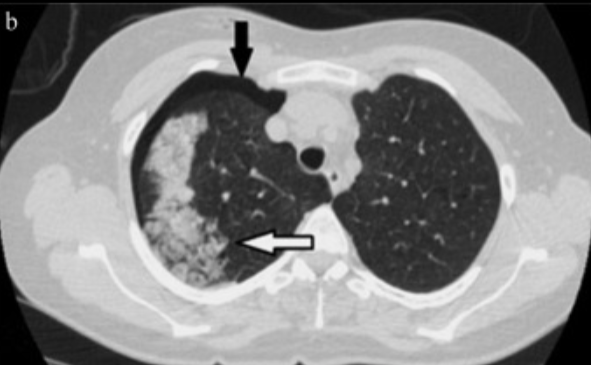
\includegraphics[width=0.6\textwidth]{imagenes/introduccion/complicacion.png}
    \caption{Ejemplo de neumotórax y hemorragia alveolar como complicaciones tras la realización de una biopsia pulmonar guiada por TC. Fuente: \cite{elshafee2019complications}.}
    \label{fig:intro_complicaciones_biopsia}
\end{figure}

La aparición de estas complicaciones puede depender de múltiples factores relacionados con el paciente, la lesión y el propio procedimiento, como la presencia de enfisema, el tamaño y la profundidad del nódulo, el contacto con la pleura o el trayecto de la aguja. Por ello, disponer de herramientas capaces de estimar el riesgo antes de realizar la biopsia podría ayudar a identificar pacientes con mayor probabilidad de eventos adversos, apoyar la planificación de la intervención y favorecer una toma de decisiones más personalizada. Además, anticipar el tipo de complicación más probable podría contribuir a una mejor organización de los recursos clínicos necesarios durante el procedimiento, como la disponibilidad de material específico, medidas de monitorización adicionales o preparación transfusional en pacientes con mayor riesgo de hemorragia.

En los últimos años, la inteligencia artificial ha mostrado un gran potencial en el análisis de datos clínicos e imagen médica. Sin embargo, gran parte de la investigación en TC torácica se ha centrado en tareas como la detección de nódulos, la caracterización tumoral o la predicción del riesgo de cáncer de pulmón. En comparación, la predicción preprocedimiento de complicaciones asociadas a la biopsia pulmonar ha recibido una atención mucho menor. Esta diferencia motiva el desarrollo de enfoques capaces de combinar información clínica e imagen médica para estudiar no solo si puede aparecer una complicación, sino también qué tipo de complicación es más probable.


\section{Precedentes}

Esta línea de investigación se inició en el Trabajo de Fin de Grado previo, centrado en la predicción binaria de complicaciones en biopsias pulmonares mediante inteligencia artificial. A partir de dicho trabajo se elaboró una publicación científica aceptada en la \textit{IEEE Conference on Artificial Intelligence 2026}, donde se expusieron resultados preliminares sobre el uso de variables clínicas, características radiómicas y modelos tridimensionales de aprendizaje profundo para este problema \cite{perez2026prediction}. Estos resultados mostraron que la aproximación era prometedora, especialmente en los enfoques basados en radiómica, pero también pusieron de manifiesto limitaciones importantes relacionadas con el tamaño muestral, la heterogeneidad de los datos y la capacidad de generalización de los modelos profundos.

El presente Trabajo de Fin de Máster surge como continuación natural de esa línea previa. Su motivación principal es avanzar desde un estudio preliminar con clasificación binaria hacia una formulación más completa y rigurosa del problema, incorporando una perspectiva multietiqueta, nuevos datos y técnicas avanzadas de inteligencia artificial adaptadas a las particularidades del contexto clínico, como el \textit{Positive-Unlabeled Learning} o el \textit{Subgroup Discovery}. El objetivo no es únicamente mejorar la capacidad predictiva, sino también contribuir a la caracterización de las complicaciones asociadas a las biopsias pulmonares, analizando qué información resulta más útil, qué patrones pueden identificarse en los datos, qué limitaciones metodológicas condicionan el aprendizaje en una cohorte clínica reducida y cómo obtener resultados robustos, trazables e interpretables en un contexto médico sensible.

\section{Propuesta}
\textcolor{red}{ Multietiqueta (realmente los tipos es lo que le interesa de verdad a los medicos, no solo si va a haber o no complicacion). Hacerla cuando este todo hecho.} 


\section{Objetivos}

\textcolor{red}{Revisarlos (Son los que se pusieron en el formulario al hacer la propuesta de tfm):}

\begin{itemize}
    \item Abordar el problema de predicción multimodal y multietiqueta de complicaciones en biopsias pulmonares con técnicas avanzadas de Inteligencia Artificial y análisis de datos.
    \item Analizar en profundidad las fuentes de información disponibles para determinar la relevancia de variables clínicas, radiómicas e imagen médica en la capacidad predictiva de los modelos.
    \item Explorar metodologías avanzadas de aprendizaje automático adaptadas a las particularidades del problema, como pueden ser desbalanceo de clases, posible incertidumbre en las etiquetas o identificación de subgrupos relevantes de pacientes, entre otros.
    \item Diseñar y evaluar modelos predictivos explicables, comparando su rendimiento y su capacidad de proporcionar interpretaciones útiles en un entorno clínico.
    \item Extraer conclusiones clínicas y metodológicas que ayuden a comprender mejor el problema y orienten futuras líneas de investigación.
\end{itemize}



\section{Planificación}

La planificación del trabajo se organizó en un periodo de seis meses, desde marzo hasta agosto de 2026. Durante este tiempo se estructuraron las tareas en varias fases principales: revisión bibliográfica y formación técnica, desarrollo del marco teórico y estado del arte, análisis exploratorio y preprocesamiento de los datos, diseño de modelos, experimentación y redacción de la memoria.

En las primeras semanas se priorizó la revisión de literatura y la familiarización con las herramientas necesarias para el tratamiento de datos clínicos e imagen médica. Posteriormente, se abordó el análisis exploratorio de los datos y el diseño de las estrategias de preprocesamiento. A partir de abril y mayo comenzó el desarrollo de los distintos enfoques de modelado, incluyendo radiómica, modelos de aprendizaje profundo y técnicas avanzadas como \textit{Positive-Unlabeled Learning} y \textit{Subgroup Discovery}. La fase experimental se extendió durante la mayor parte del proyecto, ya que fue necesario comparar distintas configuraciones, ajustar los experimentos y analizar los resultados obtenidos.

Para visualizar la distribución temporal de estas tareas, en la Figura~\ref{fig:planificacion} se muestra el diagrama de Gantt del proyecto.

\begin{figure}[!htbp]
    \centering
    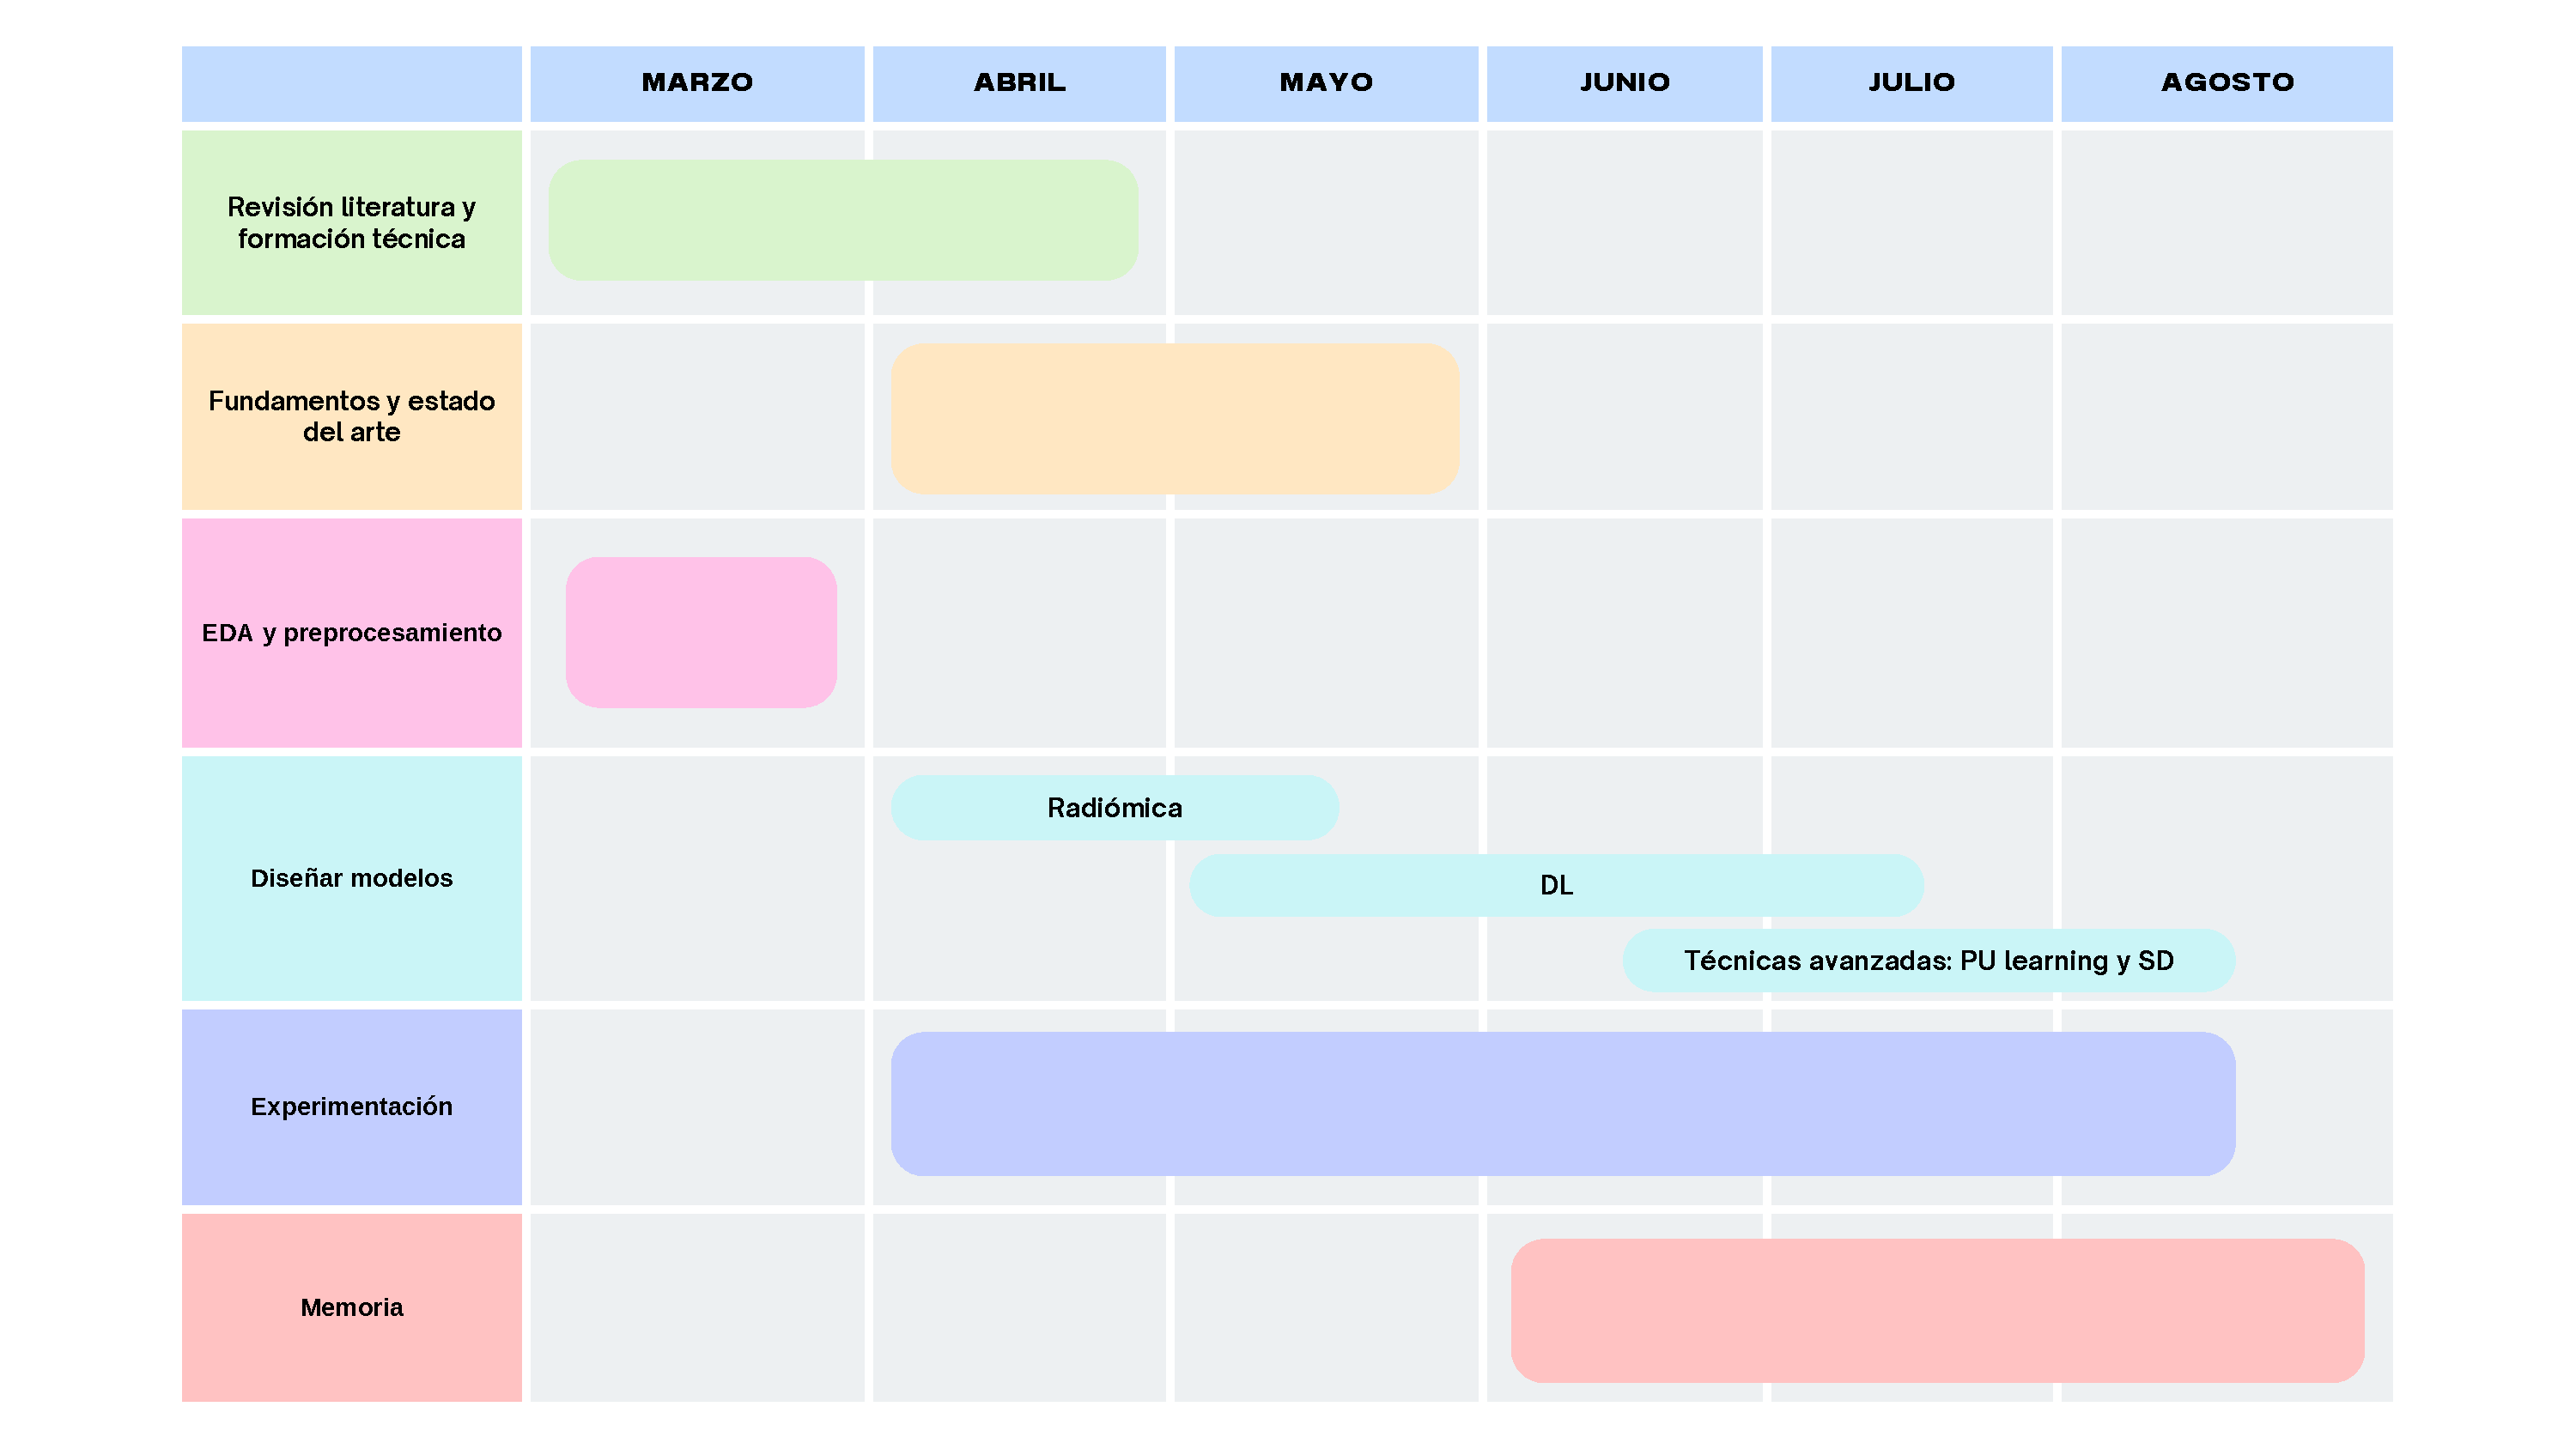
\includegraphics[width=1\textwidth]{imagenes/introduccion/gantt.pdf}
    \caption{Diagrama de Gantt del proyecto.}
    \label{fig:planificacion}
\end{figure}

Como se observa en la planificación, varias fases se desarrollaron de forma solapada. En particular, la experimentación avanzó en paralelo con la redacción de la memoria, permitiendo incorporar progresivamente los resultados y ajustar la discusión conforme se completaban los distintos bloques experimentales.



\section{Estructura de la memoria}
\textcolor{red}{A definir cuando este acabada.}



% \section{Bibliografía fundamental?}